\subsection{Base Concepts}

From the conclusion about the base concepts on (EMMA-SOTA), it is clear that
rail based ideas are the simplest solutions. So, focusing on rail concepts, here it's
explored three different ones, differentiated mainly by its movement elements.
They were all designed withstand the dynamic efforts that can cause vibration and
elevated tensions.


$\bullet$~\textbf{Prismatic-Rotacional-Rotacional Base (P-R-R):}
  
  This concept is composed of three degrees of freedom: one prismatic and two
  rotational. The prismatic joint is simply the rail, it shall be aligned with
  the runners rotational axis, being responsible for bringing the arm to the
  region near the blade. The first rotational joint is perpendicular to the
  rail, enabling the arm to be positioned even closer to the blade. The second
  rotational joint can lift the arm for it to reach more distant parts of the
  blade. Together the two rotational joints help to extend the arm's reach as
  show in the figure \ref{fig::base_prr}.

% Neste conceito estudou-se a possibilidade de utilizar uma base com $3$ graus
% de liberdade: um prismático e dois rotacionais. O prismático seria composto
% por um trilho alinhado e paralelo ao eixo da turbina que transportaria o robô
% até a região próxima a pá. Uma junta rotacional e com eixo vertical orientaria
% a base nesta direção e uma junta perpedincular à primeira faria o
% posicionamento da base do robô para então iniciar o processo de revestimento.
% A figura~\ref{fig::base_prr} ilustra este conceito.
    
  \begin{figure}[h!]
   \centering
   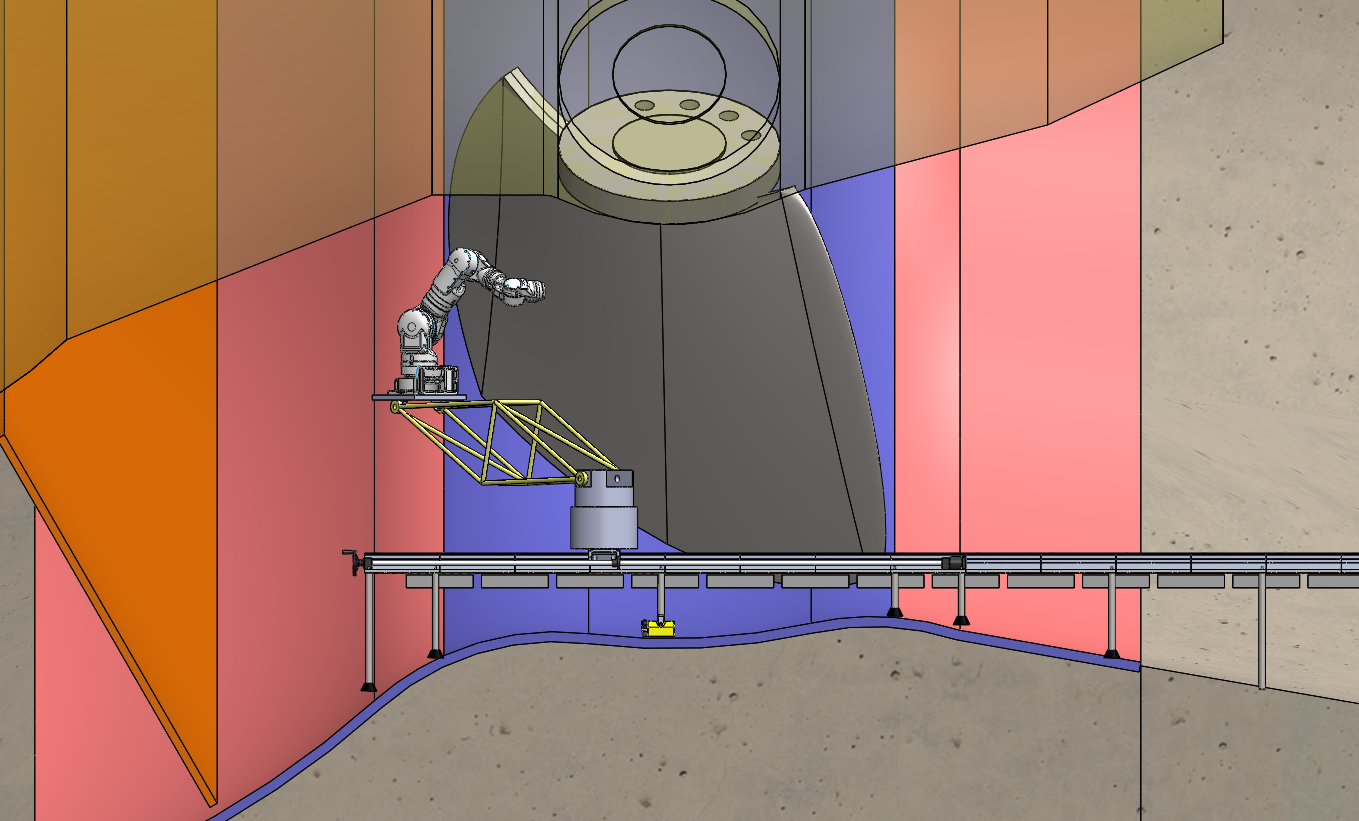
\includegraphics[width=0.8\columnwidth]{figs/bases/base_prr}
   \caption{Prismatic-Rotacional-Rotacional Base}
   \label{fig::base_prr}
\end{figure}

%   A vantagem deste conceito é conferir um alcance grande ao manipulador através
%   da base, permitindo que este possa ser de menor alcance próprio, mas ao mesmo
%   tempo mais leve.
  
  The downside of this approach was revealed by further kinematic simulations,
  where the result showed that the maneuverability of the basis is reduced in
  the small space between blades and even that there were some impossible
  configurations depending on the choice of the arm.
  
%   Porém, devido à configuração de juntas e pelos resultados encontrados no
%   estudo cinemático, a manobrabilidade desta base seria reduzida naquele espaço,
%   havendo posicionamentos difíceis de serem alcançados, ou até impossíveis
%   dependendo do manipulador escolhido.
  
$\bullet$~\textbf{Prismatic Base (P):}

  The Prismatic base is just the rail. The ideia here is instead of getting the
  arm closer to the blade, getting the blade closer to the arm, in the sense
  that the base will remain static while the runner is rotated. For it to work
  the runner must be able to rotate, so the rail has a removable section as
  figure \ref{fig::base_p} shows.
  
  The envisioned procedure for the positioning the arm goes as follow:
  \begin{enumerate}
    \item The rail is placed and fixed along the direction of the runner's axis
    (there must be no blade positioned on the way of the rail);
    \item the arm is moved on the rail to a
  position in one of the two sides of the blade (figure \ref{fig::base_p} shows the arm positioned behind the blade, but it could be
  in front of it);
  	\item The section of the rail that obstructs the rotation of the runner is
  	removed;
  	\item \label{hc} The runner is rotated so the some yet uncoated part of the
  	blade to be processed is right in front of the arm;
  	\item The arm hardcoats the region of the blade in its reach, if there are is
  	uncoated parts of the blade return to step \ref{hc}; 
       
  \end{enumerate}
  
%   Este conceito consiste de um trilho (junta prismática) para o transporte do
%   manipulador desde a escotilha até o ponto de interesse para revestimento na
%   face anterior ou posterior da pá. Quando posicionado, remove-se a seção do
%   trilho na direção que obstrui a rotação do rotor. Neste conceito, adiciona-se
%   um grau de liberdade ao sistema utilizando a própria rotação do rotor,
%   posicionando a pá em relação ao robô. A base mecânica então forneceria apenas
%   movimento no trilho na direção do eixo da turbina, deixando fixas as outras
%   direções. O procedimento para o revestimento seria o posicionamento do rotor,
%   deixando a região a ser processada ao alcance do manipulador; o posicionamento
%   do robô no trilho, em relação a pá; a ancoragem do robô no ambiente; e o
%   revestimento da região possível para aquela posição.
%   Repete-se então este procedimento até ter toda a face processada e
%   posiciona-se a próxima pá para revestimento, sem necessidade de mover ou
%   desmontar a base do robô até todas as faces daquele lado estarem completas.  A
%   figura~\ref{fig::base_p} ilustra este conceito.
  
  \begin{figure}[h!]
   \centering
   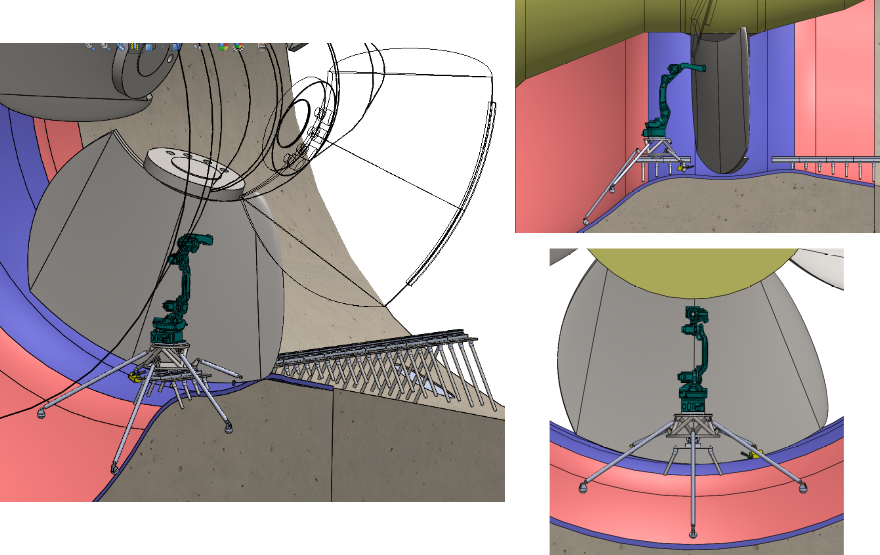
\includegraphics[width=0.8\columnwidth]{figs/bases/base_p}
   \caption{Prismatic Base}
   \label{fig::base_p}
\end{figure}


  The kinematic constrains were analized assuming the use of the Motoman's
  MH$12$ arm and sugested that it is able to hardcoalt the full vertical
  extension of the blade.
  
  The simulations also unveil some of the difficulties, a lot of diferent
  positions of the blade are necessary to hardcoat it. There are also safety
  issues that must be taken into account, e.g. the runner can only be manually
  rotated in UHE Jirau, thus it is not a very precise positioning. The personal
  must follow safety procedures to ensure low risk, for the people and
  equipament around, while rotating the runner. These concerns reduce the
  practical aplication of this solution under the an operational point of view. 

  
%   Este conceito foi estudado para o manipulador MH$12$, que de
%   acordo com a análise cinemática consegue processar toda a extensão vertical. Para outros
%   manipuladores, seria necessário incluir uma junta prismática, adicionando um
%   grau de liberdade, na direção vertical.
%   
%   A análise cinemática também demonstrou que seriam necessárias muitas posições
%   do rotor para completar uma face da pá. Há inclusive dificuldades operacionais e
%   de segurança no procedimento de rotação do rotor que devem ser considerados. O
%   rotor só pode ser girado manualmente, não fornecendo precisão no
%   posicionamento da pá em relação a base. Por ser uma tarefa manual, deve-se ter
%   procedimentos adequados de segurança para preservar tanto o operador quanto os
%   equipamentos próximos. Estas preocupações tornam a solução pouco prática sob o
%   ponto de vista operacional.

$\bullet$~\textbf{Prismatic-Rotacional-Prismatic Base (P-R-P):}



  Similar to the P-R-R design, in the P-R-P the first joint is the rail and the
  second joint is a rotational joint perpendicular to the rail. The diference
  lies on the third joint, it is a second rail seen as a prismatic joint. The
  purpose behind this concept is to position the second rail roughly parallel to
  a blade (figure \ref{fig::base_prp}). This configuration  allow the arm to be
  placed near any part of the blade without changing the fixation points (as it
  is too wide to be processed from a single position of the arm) by moving along the second rail.
  
%   Este conceito consiste de uma base composta por um trilho primário (junta
%   prismática $1$), uma plataforma de base pivotada por mancal e rolamentos entre
%   o trilho primário e secundário (junta rotacional) e um trilho secundário
%   (junta prismática $2$). Montado o trilho primário alinhado ao eixo da turbina
%   a base rotacional sobre o trilho primário, fixa-se o robo sobre a base
%   rotacional. Esta base permitrá a montagem do trilho secundário apenas quando o
%   robô atingir a região de interesse para revestimento. Quando posicionado o
%   manipulador, monta-se então o trilho secundário alinhado ao plano paralelo a
%   face da pá e ancora-se a base no ambiente. Desta forma, o robô pode-se
%   movimentar ao longo de toda a extensão da pá por meio do trilho secundário e
%   também se aproximar e se afastar da superfície da pá, por meio do trilho
%   primário. A figura~\ref{fig::base_prp} ilustra este conceito.

% \begin{figure}[h!]
%    \centering
%    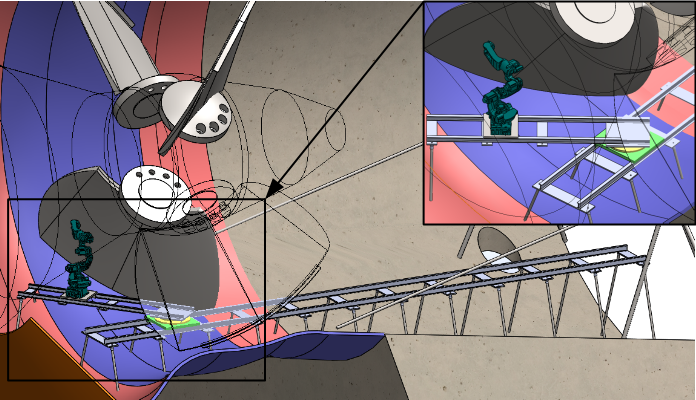
\includegraphics[width=0.9\columnwidth]{figs/bases/base_prp}
%    \caption{Prismatic-Rotacional-Prismatic Base}
%    \label{fig::base_prp}
% \end{figure}

  Futher geometric analyzes showed that the blades (????) must be rotated by
  $30^o$ at least, otherwise it can shock with the first rail. When the runner
  is rotate for positining the next blade to be processed, it is necessary to
  unmount the part of the rail that gets in the way of the blades. On the other
  hand, for the two sides of the same blade it is only needed for the second
  rail to be moved, along the first rail, to the other side of the blade.
  Moving or umounting/mouting in any rail means that its attachment points need
  also to be repositined. 
  
  Despite some operational complexities, it is a mechanically
  simpler solution and does not result in safety concerns.
  
%   Desta forma, o rotor deve estar girado em, no mínimo $30^o$ para não haver
%   contato com o trilho primário. A análise cinemática será realizada para
%   encontrar a melhor configuração de juntas da base que permite ao robô se
%   movimentar nos graus de liberdade da base, sem alterar o posicionamento do
%   rotor e, assim, cobrir uma face inteira da pá. Para a repetição do processo
%   nas outras pás do lado da sucção da turbina, é necessária a desmontagem do
%   trilho secundário, o recuo do robô e desmontagem de parte do trilho primário,
%   permitindo o giro do rotor para a pá seguinte.
%   Para as faces do lado de adução, não é necessária a desmontagem parcial do
%   trilho primário. 
